\section{Layout}

\begin{frame}{Columns, blocks and figures}
  \begin{columns}
    \begin{column}{0.5\textwidth}
      \begin{block}{Block}
        Standard block.
      \end{block}
      \begin{alertblock}{Alert block}
        Something important.
      \end{alertblock}
      \begin{exampleblock}{Example block}
        Something illustrative.
      \end{exampleblock}
    \end{column}
    \begin{column}{0.45\textwidth}
      \begin{figure}
        \centering
        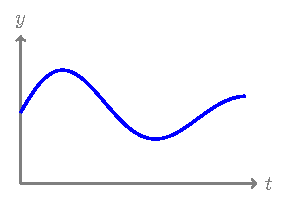
\includegraphics[width=\linewidth]{diagram}
        \caption{A PDF figure found via \texttt{\textbackslash graphicspath}.}
      \end{figure}
    \end{column}
  \end{columns}
\end{frame}

\begin{frame}{Tables}
  \centering
  \begin{tabular}{lrrr}
    \toprule
    Solver & Steps & Time (\si{\milli\second}) & Error \\
    \midrule
    Euler & 1000 & 12.1 & $1.2\times10^{-2}$ \\ \pause
    Heun  & 500  & 9.8  & $3.4\times10^{-4}$ \\ \pause
    RK4   & 100  & 4.2  & $\mathbf{2.1\times10^{-7}}$ \\
    \bottomrule
  \end{tabular}

  \bigskip
  \begin{quote}
    ``Make it work, make it right, make it fast.'' --- Kent Beck
  \end{quote}
\end{frame}

\begin{frame}{Text}
  \begin{description}
    \item[Emphasis] \emph{emph}, \textbf{bold}, \textit{italic}, \textsc{Small Caps}, \texttt{mono}, \underline{under}
    \item[Colour] \textcolor{blue}{blue}, \textcolor{red!70!black}{dark red}, \colorbox{yellow!30}{boxed}, \alert{alert}
    \item[Sizes] {\tiny tiny} {\small small} {\large large} {\Large Large}
    \item[Accents] Erd\H{o}s, Poincar\'e, G\"odel, \v{C}ech, Fran\c{c}ois, \AA ngstr\"om
    \item[Symbols] \checkmark\ \textdegree C \ldots\ \copyright\ 2026 --- en--dash
  \end{description}
\end{frame}
